\documentclass[../manuale_sviluppatore.tex]{subfiles}

\begin{document}
Il prodotto HD-Viz è stato progettato con un occhio di riguardo verso l'estensibilità dello stesso; 
le modalità di estensione del prodotto tenute particolarmente in considerazione sono le seguenti:
\begin{itemize}
	\item aggiunta di visualizzazioni ex-novo;
	\item aggiunta di funzionalità alle visualizzazioni preesistenti.
\end{itemize}
Di seguito saranno trattate entrambe le tipologie di estensione e sarà spiegato come poterle 
realizzare nel prodotto HD-Viz.

\subsection{Aggiunta di visualizzazioni}
Per poter aggiungere una visualizzazione sarà necessario implementare i seguenti tipi:
\begin{itemize}
	\item modello della visualizzazione;
	\item presenter della visualizzazione;
	\item eventuali component specifici della visualizzazione;
	\item factory per la creazione del modello;
	\item factory per la creazione del presenter e dei componenti.
\end{itemize}

Innanzitutto è necessario implementare il modello della visualizzazione, esso dovrà estendere 
\emph{GraphModel} e in base alle funzionalità che saranno rese disponibili dovrà implementare le 
interfacce relative ai componenti che utilizzerà. All'interno del modello dovranno essere mantenuti 
tutti i dati relativi alla configurazione della visualizzazione e delle strutture dati su cui esso 
dipende.

\begin{figure}[H]
	\centering
	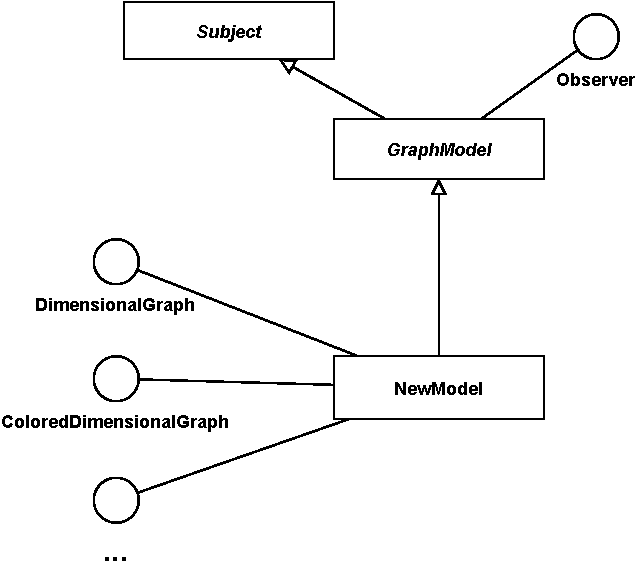
\includegraphics[width=10cm]{img/extendModel.pdf}
	\caption{Estensione di GraphModel}
\end{figure}

Successivamente bisognerà implementare il presenter della visualizzazione, esso dovrà estendere 
\emph{GraphPresenter} e per ciascuna funzionalità della visualizzazione dovrà implementare un metodo 
che la implementi. Il presenter dovrà iscriversi agli eventi di suo interesse presso il modello e 
dovrà implementare il metodo update con una risposta coerente per ciascuna tipologia di evento a cui 
esso si è iscritto.\\

\begin{figure}[H]
	\centering
	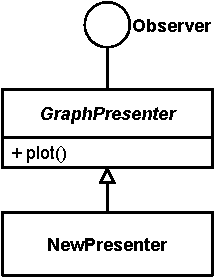
\includegraphics[width=3cm]{img/extendPresenter.pdf}
	\caption{Estensione di GraphPresenter}
\end{figure}


Nel caso siano necessari dovranno essere implementati component specifici della visualizzazione per 
permettere delle funzionalità non ancora presenti in HD-Viz, per ulteriori dettagli si rimanda a 
\refSec{sub:funzionalita}.\\

Infine sarà necessario implementare una factory che crei il modello del grafico, ed implementare 
un'ulteriore factory per la creazione del presenter e delle componenti della visualizzazione.

\begin{figure}[H]
	\centering
	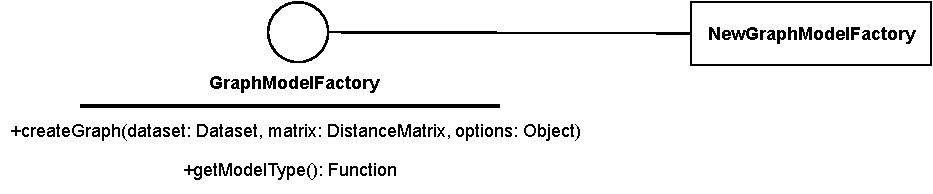
\includegraphics[width=12cm]{img/extendModelFactory.pdf}
	\caption{Estensione di GraphModelFactory}
\end{figure}

\begin{figure}[H]
	\centering
	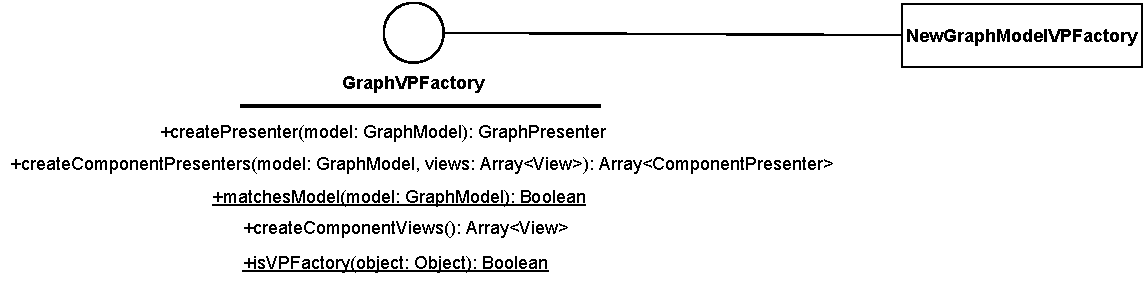
\includegraphics[width=15cm]{img/extendVPFactory.pdf}
	\caption{Estensione di GraphVPFactory}
\end{figure}


\subsection{Aggiunta di funzionalità a visualizzazioni preesistenti}
\label{sub:funzionalita}

Per poter aggiungere funzionalità a visualizzazioni preesistenti è necessario svolgere le seguenti 
operazioni:
\begin{itemize}
	\item estendere il modello della visualizzazione;
	\item estendere il presenter con i metodi che implementino la funzionalità;
	\item implementare il component per gestire la funzionalità;
	\item aggiornare le factory;
\end{itemize}

Se necessario, il modello della visualizzazione alla quale si desidera aggiungere una 
funzionalità deve essere esteso con le informazioni necessarie per gestire la funzionalità e i 
metodi per modificare tali informazioni.\\

Inoltre sarà necessario aggiungere dei metodi che implementino la funzionalità nel presenter della 
visualizzazione, di modo che essi possano essere richiamati in risposta ad un determinato evento al 
quale il presenter dovrà essere iscritto durante la sua costruzione.\\

I metodi che verranno aggiunti nel modello implementeranno una nuova interfaccia, dalla quale un 
eventuale component dipenderà per modificare le proprietà della visualizzazione inerenti alla 
funzionalità aggiunta. Sarà quindi necessario all'occorrenza definire un nuovo component per la 
gestione della funzionalità, e aggiornare di conseguenza la factory della visualizzazione che ha il 
compito di creare il presenter e i components.

\end{document}
